\chapter{Implementa��o}
\outlineon=0


\outline{
  Descrever o processo de Implementa��o no tinyos (libs, organiza��o do c�digo e TEPs).
  
}

Este cap�tulo trata sobre o sistema operacional TinyOS a linguagem nesC e os dispositivos de \textit{hardware}. Aspectos importantes de sua arquitetura para a implementa��o de um protocolo de sincroniza��o. 



\section{Mote}\label{sec:mote}

O termo \textit{mote} � utilizado para se referir ao dispositivo que � n� em uma rede de sensores sem fio, foi introduzido por pesquisadores da Universidade de Berkeley \cite{culler2002mica} no in�cio da d�cada de 90, assim, constantemente podemos encontrar refer�ncias como ``Berkeley Mote'' para designar estes dispositivos de rede, independente do fabricante. 

O MicaZ � um \textit{mote} dispon�vel comercialmente e amplamente utilizado em pesquisas acad�micas. Possui um processador de 4 MHz com 8 \textit{bits}, mem�ria de 128 kB. A diferen�a comparado a um computador com a capacidade similar do in�cio da d�cada de 1980, como o 8088, � o baixo consumo de energia que varia de 15 $\mu$A no modo de economia at� 8 mA em execu��o. Outro componente significativo � o r�dio, esses dispositivos possuem transmissores com frequ�ncia de 2.4 GHz e taxa de dados de 250 kbps, usam a estrat�gia de acesso ao meio CSMA/CA, conseguindo transfer�ncias de 40.000 bps.


\begin{table}[h]
\centering
\begin{tabular}{lcc}
\hline
\textbf{Item}         & \textbf{MicaZ}              & \textbf{Iris}\\
\hline
Processador           & ATMega 128L 8MHz            & ATmega1281 16MHz                                                                  \\
\textit{Flash}        & \multicolumn{2}{c}{128 kB}                                                                                                                                                           \\
Mem�ria Dados         & \multicolumn{2}{c}{512 kB}                                                                                                                                                           \\
EEPROM                & \multicolumn{2}{c}{4 kB}                                                                                                                                                             \\
ADC                   & \multicolumn{2}{c}{10 bit}                                                                                                                                                           \\
\textit{Chip} de R�dio         & CC2420                     & RF230                                                                             \\
Frequ�ncia do R�dio   & \multicolumn{2}{c}{2.4 GHz}                                                                                                                                                          \\
Taxa de Transfer�ncia & \multicolumn{2}{c}{250 kbps}                                                                                                                                                         \\
Voltagem de Opera��o  & \multicolumn{2}{c}{3,6 - 2,7}                                                                                                                                                        \\
Consumo de Energia    & \begin{tabular}[c]{@{}c@{}}RX 19,7 mA\\ TX 17,4 mA\\ \textless 15 $\mu$A (dormindo)\end{tabular} & \begin{tabular}[c]{@{}c@{}}RX 16 mA\\ TX 17 mA\\ 8 $\mu$A (dormindo)\end{tabular}\\
\hline
\end{tabular}
\caption{Especifica��es de \textit{hardware} dos \textit{motes}}
\label{tab:micazxiris}
\end{table}

A jun��o destas caracter�sticas, fornecem recursos que tornam o \textit{mote} uma boa op��o para diversas aplica��es, a capacidade de computa��o o consumo de energia trazem a flexibilidade para implanta��o destes equipamentos em RSSF, a Tabela \ref{tab:micazxiris} cont�m as especifica��es dos \textit{hardwares} utilizados. 


\section{Sistema Operacional}

\outline{
\begin{itemize}
 \item Gerencia de mem�ria. Gerenciamento energ�tico. Redes. Linguagem. Manipula��o de interrup��es. Programa��o baseada em eventos.
\end{itemize}    
}



O desenvolvimento do FTSP+ foi realizado utilizando o sistema operacional TinyOS, que � um SO bem difundido na �rea de redes sensores sem fio \cite{levis2004tinyos}. O TinyOS n�o � um sistema operacional convencional, em que se instala completamente no sensor. O sistema apresenta-se como um arcabou�o de um conjunto de componentes, reutiliz�veis e que permite o desenvolvimento de aplica��es para sistemas embarcados em conjunto com o SO. Esses componentes s�o separados por fun��es caracter�sticas, no momento de construir a aplica��o somente os componentes especificados ser�o integrados na aplica��o final, mantendo o uso minimal de recursos. 

Com a limita��o de recursos nos dispositivos sensores o TinyOS conta com pouco menos de 400 \textit{bytes} de tamanho, � um sistema baseado em eventos, com suporte a concorr�ncia, eventos ass�ncronos e comandos. Um programa em TinyOS possui a abstra��o dos componentes em um modelo de grafo, como vemos na Figura \ref{fig:diagrama_componentes}.


As aplica��es e o pr�prio sistema operacional s�o escritos em nesC (\textit{networked systems C}) \cite{gay2003nesc} um dialeto da linguagem C. Esta linguagem d� o suporte a arquitetura de componentes e orienta��o a eventos. � otimizada para reduzir o consumo de mem�ria e tem primitivas que previnem problemas de baixo n�vel, como por exemplo, condi��o de corrida. No desenvolvimento existe a separa��o da organiza��o dos componentes e programa��o das interfaces, os componentes s�o conectados (\textit{wired}) juntos em um arquivo de aplica��o, j� o c�digo dos eventos e tarefas s�o feitos em um arquivo de constru��o.


%Como o TinyOS tem o c�digo aberto, � poss�vel alter�-lo e criar ou estender suas funcionalidades.

Programas em nesC s�o constru�dos por itens definidos separadamente e ent�o conectados de forma explicita para juntar todos em uma unidade \cite{levis2009tinyos}. A seguir defini��es importantes sobre essas caracter�sticas:

\begin{itemize}
 \item Componentes e interfaces: Um programa em nesC � um conjunto de componentes ligados entre si. O componente fornece interfaces que s�o respons�veis pela comunica��o bidirecional entre os componentes, as interfaces fornecem comando e eventos.
 
 \item Implementa��o: A implementa��o pode ser dividida em duas partes no nesC, uma chamada \textit{modules} e outra \textit{configuration}. Em \textit{modules} � implementado as interfaces, j� em \textit{configuration} � usado para juntar os componentes conectando suas interfaces.
 
 \item Modelo de concorr�ncia: Define como os componentes interagem entre suas execu��es. Temos dois tipos de tarefa, que s�o a tarefa (ou \textit{task}) propriamente dita e eventos de dispositivos. Quando uma tarefa � enviada para execu��o ela roda at� completar, n�o fazendo preemp��o. Os eventos de dispositivos s�o como as tarefas, s� que s�o geradas como respostas a eventos.
\end{itemize}



\begin{figure}[h]
\center
\subfigure[fig:arq_trad][Arquitetura Tradicional]{\includegraphics{./figuras/arquitetura_tradicional.eps}}
\qquad
\subfigure[fig:arq_tinyos][Arquitetura Tinyos]{\includegraphics{./figuras/arquitetura_tinyos.eps}}
\caption{Compara��o das arquiteturas}\label{fig:comp_arq}

\end{figure}


A arquitetura do TinyOS difere das arquiteturas cl�ssicas, a Figura \ref{fig:comp_arq} ilustra a organiza��o dos dois tipos. No cen�rio das RSSF sistemas operacionais tradicionais apresentam as seguintes restri��es: grande necessidade de armazenamento e mem�ria, maior consumo de energia, custo computacional das trocas de contexto e uso mem�ria virtual entre outros. O TinyOS simplifica sua arquitetura para tornar-se mais espec�fico para suas aplica��es: n�o possui \textit{kernel}, a manipula��o do \textit{hardware} � realizado diretamente, sem gerenciamento de processos tem apenas um processo de tempo real, n�o utiliza mem�ria virtual, ao inv�s disso, tem um �nico espa�o de endere�o f�sico linear. A figura do escalonador representa uma grande mudan�a entre os paradigmas, o TinyOS coloca seu \textit{scheduler} no topo da arquitetura, assim uma aplica��o � o resultado da jun��o de seus componentes com o escalonador. 


\section{Diagramas e Componentes}\label{sec:dia}

\outline{
  O Tinyos tem o recurso de componentes para disponibilizar seus mais diversos recursos, descrever os componentes relevantes para o trabalho e os componentes resultantes das altera��es.
}

O TinyOS foi desenvolvido seguindo um conjunto de diretrizes, chamado de TEP (TinyOS Enhancement Proposals) que orientam as modifica��es no n�cleo do seu c�digo, tamb�m � utilizado para guiar a cria��o de novas funcionalidades. Podemos citar as seguintes TEPs \cite{tinyos133, tinyos132, tinyos102} com defini��es importantes para a implementa��o do FTSP+:

\begin{itemize}
 \item TEP 102: Prop�e a estrutura dos \texttt{Timers} (controladores do rel�gio) e suas propriedades de precis�o, acur�cia e tamanhos.
 \item TEP 132: Descreve o mecanismo de \textit{timestamp} no n�vel de acesso ao meio. A funcionalidade que fornece o tempo de envio e recebimento de uma mensagem no processo de comunica��o.
 \item TEP 133: Descreve o funcionamento do mecanismo das mensagens de sincroniza��o de tempo, como os tempos s�o convertidos do tempo do emissor para o do receptor e como s�o tratados nas pilhas de protocolos.
\end{itemize}

Os \textit{Timers} no TinyOS fornecem precis�es listadas na Tabela \ref{tab:precision}, todas as precis�es s�o bin�rias, ou seja, 1s cont�m 1024 milissegundos bin�rios. A acur�cia dependente de qu�o bem o dispositivo fornece de seu rel�gio, como vimos anteriormente os rel�gios s�o afetados pelas limita��es de seu \textit{hardware}. Assim um rel�gio de um \textit{mote} que roda a 7.37MHz, tem valor real do rel�gio variando muito pr�ximo desse valor. Os tamanhos s�o basicamente 8, 16, 32 e 64 \textit{bits}, sendo 32 \textit{bits} o tamanho indicado para representa��o dos tempos dos componentes.

\begin{table}[h]
\centering
\begin{tabular}{lccc}
Nome & TMilliC & T32kHz & TMicroC \\
\hline
Frequ�ncia & 1,024 Hz & 32,768 Hz & 0.9216 MHz \\
\hline
Precis�o & 1024 ticks/s & 32768 ticks/s & 1048576 ticks/s \\
\hline
Periodo & 976 ms & 30.518 $\mu s$ & 1.084 $\mu s$
\end{tabular}
\caption{Precis�es dos \textit{Timers} no TinyOS}
\label{tab:precision}
\end{table}%alemao


O FTSP+ foi elaborado utilizando os \textit{motes} Iris e Micaz \cite{Iris2007, Micaz}, e constru�do sobre a implementa��o j� existente do FTSP. A Figura \ref{fig:diagrama_componentes} apresenta os componentes utilizados pelo FTSP+, a altera��o descrita na Se��o \ref{sec:mod} est�o presentes no componente central da imagem o \texttt{TimeSyncP}.



\begin{figure}[h]
 \centering
 %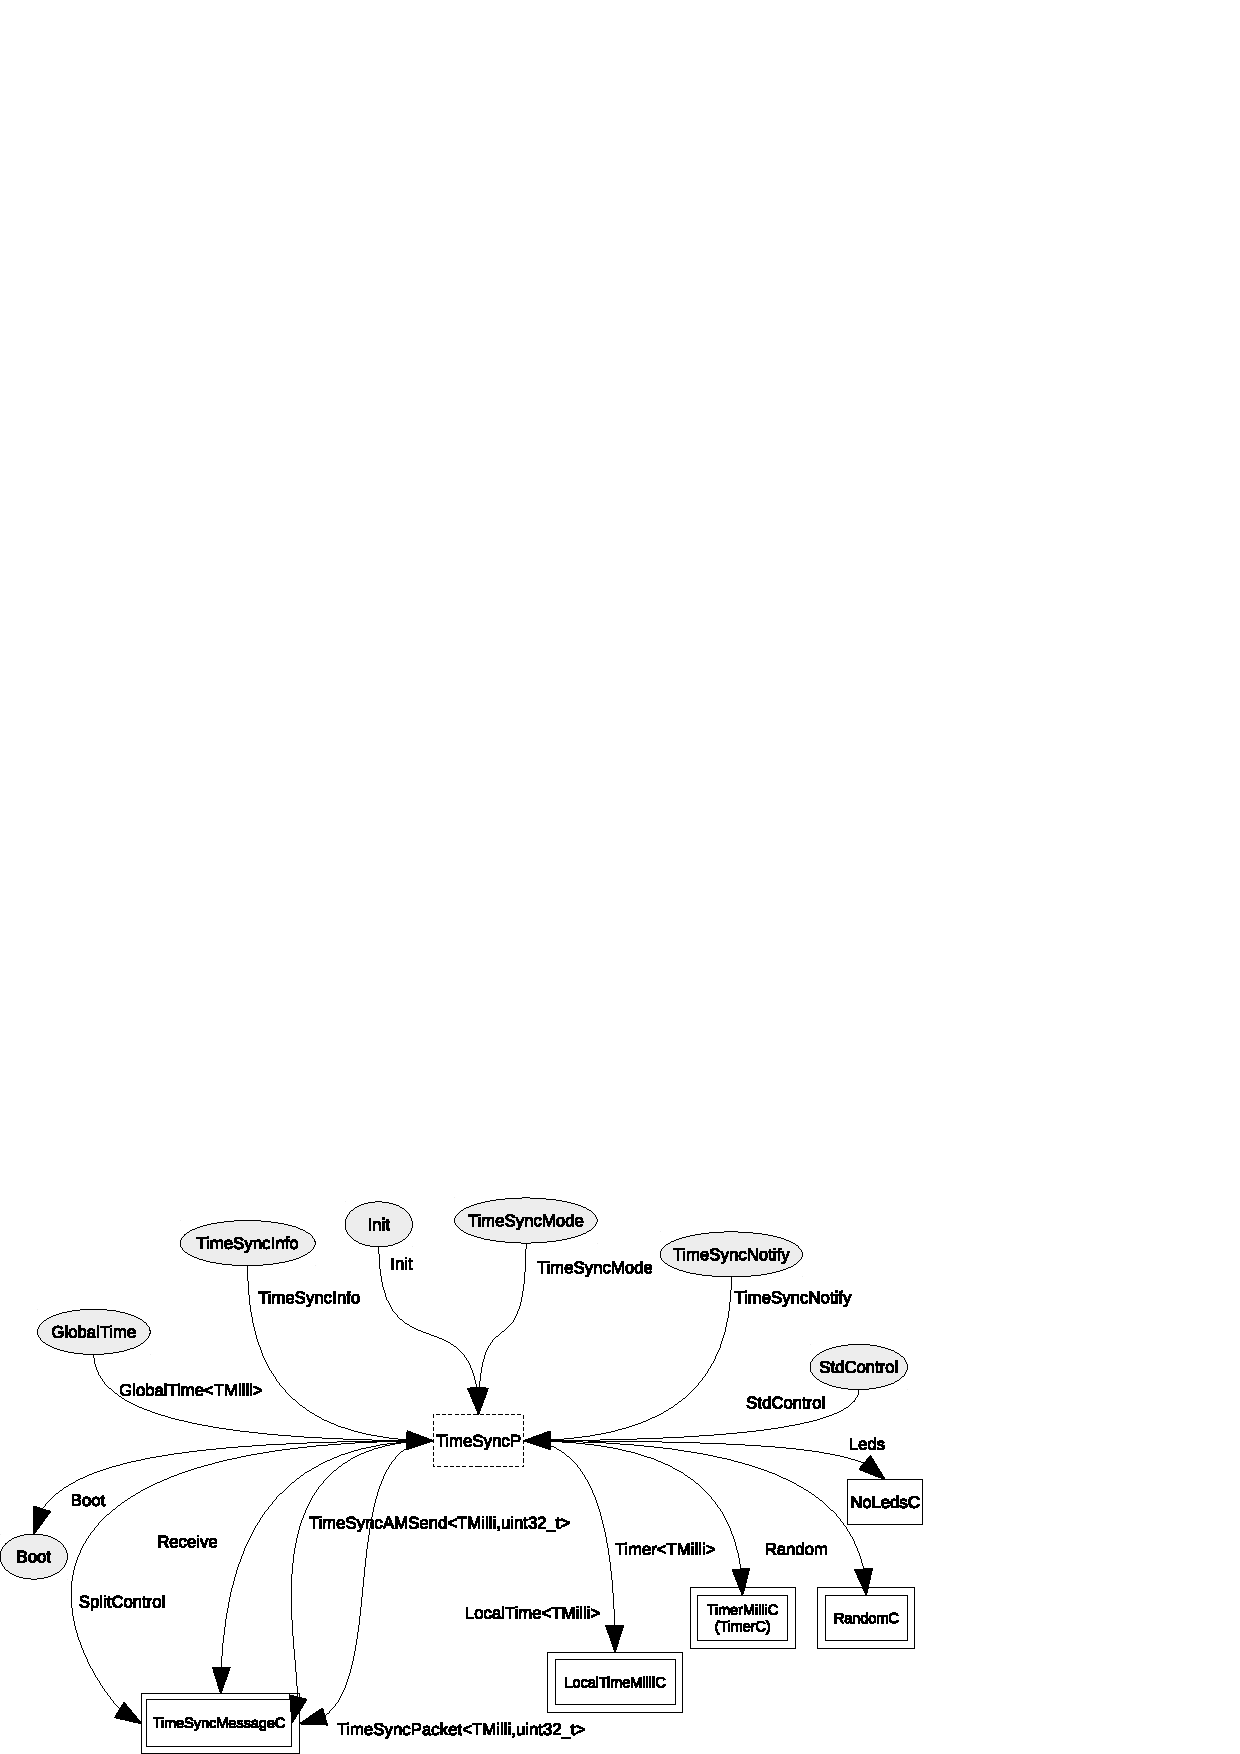
\includegraphics[width=23cm, angle=90]{./figuras/time.png}
 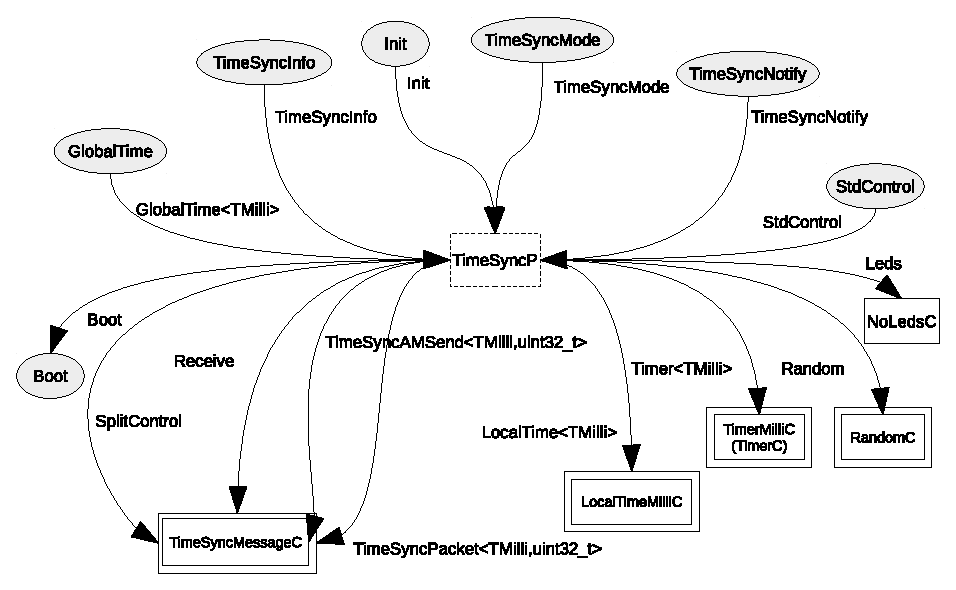
\includegraphics{./figuras/time.eps}
 % tos.lib.ftsp.TimeSyncC.png: 1177x293 pixel, 72dpi, 41.52x10.34 cm, bb=0 0 1177 293
 \caption{Diagrama de Componentes do FTSP+}
 \label{fig:diagrama_componentes}
\end{figure}

O \texttt{TimeSyncP} faz parte a implementa��o original do FTSP, por�m foi o �nico componente modificado. O FTSP usa uma mensagem de sincroniza��o com informa��es como o ID do n� raiz da rede, o ID do n� que est� enviando a mensagem de sincroniza��o, um n�mero de sequ�ncia da mensagem e o seu \textit{timestamp}. No FTSP+ � acrescentado mais uma mensagem na comunica��o, que � a mensagem de corre��o. A estrutura da mensagem � listada a seguir:

% \begin{figure}[h]
%  \begin{Verbatim}[numbersep=1pt,frame=single]
% typedef nx_struct TimeSyncMsg
% {
%  nx_uint16_t rootID;
%  nx_uint16_t nodeID; 
%  nx_uint8_t  seqNum;
%  nx_uint32_t globalTime;
%  nx_uint32_t localTime;
% } TimeSyncMsg;
% \end{Verbatim}
% \caption{Formato da mensagem de sincroniza��o}
% \end{figure}

\begin{figure}[h]
 \begin{Verbatim}[numbersep=1pt,frame=single]
typedef nx_struct TimeSyncMsg {
 nx_uint16_t rootID;
 nx_uint16_t nodeID;      
 nx_uint8_t  seqNum;
 nx_uint32_t correction; 
} TimeSyncMsg;
\end{Verbatim}
\caption{Formato da mensagem de sincroniza��o}
\end{figure}


O mensagem conta com o \texttt{rootID}, se a mensagem tem \textit{root} com ID maior que a informa��o do \textit{root} local ela � descartada. O \texttt{nodeID} cont�m o ID de quem enviou a mensagem. O \texttt{seqNum} serve para identificar qual o \textit{timestamp} a mensagem est� corrigindo. O campo \texttt{correction} � o campo que traz a estimativa de erro do emissor e � com ele que ser� feita a corre��o dos \textit{timestamp} anteriormente recebidos.

No documento da TEP 132 \cite{tinyos132}, � fornecido uma breve descri��o sobre o padr�o de \textit{timestamps} oferecidos pela interface \texttt{PacketTimeStamp} que faz o acesso ao tempo de recep��o e envio de determinada mensagem.

A TEP 133 fornece a abstra��o para o mecanismo de sincroniza��o de pares. N�o prov� um sincroniza��o completa da redes, mas, com seus recursos � poss�vel implementar um servi�o de sincroniza��o completo, exemplo o FTSP, pois os componentes e interfaces utilizados em sua implementa��o est�o bem definidos em seu documento \cite{tinyos133}. 

Outro aspecto importante da TEP 133 � o seu guia de implementa��o, que compreende duas abordagens, uma em que � poss�vel mudar o \textit{payload} da mensagem durante a transmiss�o usando a interrup��o SFD dos r�dios orientados a pacote. A segunda abordagem descreve a possibilidade da sincroniza��o para plataformas em que n�o seja poss�vel a altera��o do conte�do durante a transmiss�o. Podemos verificar que o FTSP atende a primeira abordagem, j� a segunda n�o � atendida, por�m com o FTSP+ ambas as abordagens s�o acolhidas.


\begin{figure}[h]
 \centering
 \includegraphics{./figuras/arq_prot_sync.eps}
 % arq_prot_sync.eps: 0x0 pixel, 300dpi, 0.00x0.00 cm, bb=
 \caption{Arquitetura de \textit{Software} do protocolo de sincroniza��o}
 \label{fig:arq_prot_sync}
\end{figure}

Ao final temos a seguinte arquitetura de sincroniza��o resultante do FTSP+ no TinyOS, Figura \ref{fig:arq_prot_sync}. O oscilador de cristal incrementa o contador do rel�gio f�sico, que por sua vez alimenta o rel�gio l�gico, o FTSP+ usa o rel�gio l�gico (Componente \texttt{Timer}) para obter o valor do tempo local do n�, assim pode calcular seu desvio, estimar o tempo global e atualizar novamente o rel�gio, bem como, enviar e receber essas refer�ncias de tempo pelo transmissor de r�dio. As setas da imagem denotam troca de dados entre os componentes, a seta tracejada refere-se ao mecanismo do FTSP de MAC \textit{timestamp}. 

O pr�ximo cap�tulo traz experimento realizado com \textit{motes} reais, e gr�ficos estat�sticos dos resultados encontrados, os experimentos foram baseados nas t�cnicas descritas no trabalho. 







 
